\documentclass{article}
	\usepackage[margin=75pt]{geometry}
	\usepackage{multicol}
	\usepackage{fancyhdr}
	\usepackage{graphicx}
	\usepackage[none]{hyphenat}
	\usepackage[hyphens]{url}
	\usepackage{titlesec}
	\usepackage{lettrine}
	\usepackage{listings}
	\usepackage{color}
	\usepackage[utf8]{inputenc}
	\usepackage{float}
	\usepackage{wrapfig}
	\usepackage{pdfpages}
	\usepackage{pdflscape}
		\setlength{\floatsep}{0pt}
		\floatstyle{plaintop}
		\newfloat{slide}{h}{sld}
		\floatname{slide}{Slide}
	\graphicspath{ {./../Images/} }
	\pagestyle{fancy}

\setlength{\parindent}{0cm}

\begin{document}
	\sffamily
	% Header content
	\fancyhf{}
	\fancyhead[L]{\bf Max Morris\\Games Programmer\\}
	\fancyhead[C]{\bf {\Huge CV} \\ Maximo1491@hotmail.com\\}
	\fancyhead[R]{\bf MaxTheProgrammer.co.uk\\Mobile: 07896014448\\}


\newpage
\section*{}
\vspace{-3mm}
% Skills
\section*{Skills}
\vspace{-6mm}
\begin{tabular}{|  p{0.3\textwidth} | p{0.3\textwidth} | p{0.3\textwidth} |}
\multicolumn{3}{c}{ } \\ \hline  
C++  & OpenGL & DirectX \\ \hline
C\# & Visual Studio & Perforce \\ \hline
Github & HTML5 \& CSS & Javascipt \\ \hline
Python & Processing & Nintendo Switch \\ \hline
Microsft Office & iOS & Android \\ \hline
\end{tabular}
%Portfolio
\section*{Professional Portfolio}
Online portfolio available at {\bf \large www.MaxTheProgrammer.co.uk} this contains all current work both completed at university and during my free time. \\
Games programmer at {\bf \large Sports Interactive} as part of their {\bf \large Core Tech} team. Dedicated team member with a passion for video games and the games industry.

% Work Experience
\section*{Work Experience }
\subsection*{Sports Interactive, Core Tech\hfill \textbf{May 2014 - Present}}
At Sports Interactive I have been working as part of their Core Tech team, my role here is to implement functionality across all of their projects. This involved maintaining, improving, optimising and adding new functionality to the shared platform libraries across multiple platforms.
\\\\During my time here I have helped produce multiple titles on multiple platforms including Football Manager 2015 - Football Manager 2019, every version of Football Manager Touch (The iOS and Android version of the game), every version of Football Manager Switch (The Nintendo Switch version of the game) as well as maintaning libraries used by both Football Manager Mobile and Football Manager Online.
\\\\I also too a leading role in the warchild gamejam for Sports Interactive's Malkia which focused around a mother trying to keep her children alive, fed and educated throughout war torn parts of Africa.

% Education
\section*{Education}
\subsection*{Goldsmiths, University of London (September 2013 - 2014)}
\begin{tabular}{ p{0.4\textwidth} p{0.05\textwidth} p{0.5\textwidth} p{0.05\textwidth} }
	\multicolumn{2}{l}{\textbf{MSc Computer Games and Entertainment}} & \textbf{Graduated with Distinction} \\ \\
	Mathematics and Graphics 1 (C++) & 77 &	Mathematics and Graphics 2 (C++) & 78 \\
	Tools and Middleware (C++) & 65	& Business & 62 \\
	Advanced Programming (C++) & 78	& AI (C++) & 60 \\
	Intro to Programming (C++) & 68	& Physics \& Animation (HTML5 \& JS / Unity) & 70 \\
	\bf{\emph{Other noteable mentions}} \\
	Student Representative for the course. \\
	\multicolumn{4}{l}{Arranged and organised a {\bf \large Global Game Jam 2014} event held at Goldsmiths.} \\
	\multicolumn{4}{l}{Organised a {\bf \large UKIE Game Jam 2014} event held at Goldsmiths.} \\
\end{tabular}\\ 
%----------------------------------------------------------------------------------------------------------------------------------------------------------------------------------------
% Page 2
\newpage
\subsection*{}
\vspace{-3mm}
\subsection*{London Metropolitan University (September 2010 - 2013)}
\begin{tabular}{ p{0.4\textwidth} p{0.05\textwidth} p{0.5\textwidth} p{0.05\textwidth} }
	\textbf{BSc Computer Games Programming} 	& 		&	\textbf{Graduated with 1st Class} \\ 
	\bf{\emph{Year Long Modules}} \\
	Prototype Development (C++ \& DirectX)	&	A 	&	Final Project (C++ \& DirectX)	&	B \\ 
	\bf{\emph{Term Long Modules}} \\
	Artificial Intelligence (HTML5 \& JS)		& 	A 	&	Artificial Intelligence for games (C++) &		A \\
	Graphics and Imaging (C++ \& OpenGL)	& A	& Event Modelling and Simulation (C++ \& OpenGL)	& A \\
	Specialist Programming (C++)		& B	& Web Games Design and Development (HTML5 \& JS)	& A \\
	Mathematical Techniques	&	A	& C++ programming: An introduction		& A \\
	\bf{\emph{Other noteable mentions}} \\
	Student Representative for the course \\
	\multicolumn{4}{l}{Competed in the {\bf \large Brains Eden Game Jam 2013} with other students from London Metropolitan University.} \\
\end{tabular}  \\
\vspace{-6mm}
%Hobbies and Interests
\section*{Hobbies \& Interests}
\vspace{-3mm}
After work and during my weekends, I try to spend as much time as possible with my family and friends, normally either down the pub or spending the evening with a few of my mates fighting around the map in Heroes of the Storm. While current circumstances have seen my gaming sessions take a back-seat to higher priorities, I still try to spend some time playing around with some of the great games out there at the moment.

\vspace{-3mm}
% Referees
\section*{Referees}
\vspace{-3mm}
\begin{tabular}{ p{0.5\textwidth} p{0.5\textwidth}}
	\textbf{William Latham} 						& 	\textbf{Svein Kvernoey} \\
	Course Tutor 							& 	Line Manager \\
	Department of Computing						&	Technical Director \\
	Goldsmiths, University of London					&	Sports Interactive \\
	
	\textbf{Tel:}	+44(0) 20 7078 5052				&	\textbf{Tel:} N/A \\
	\textbf{E-mail:} w.latham@gold.ac.uk				& 	\textbf{E-mail:} Svein.Kvernoey@sigames.com \\
\end{tabular}

\begin{slide}[H]
\centering
\minipage{0.40\textwidth}
	\fbox{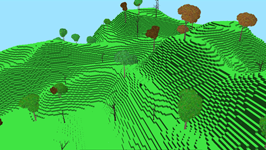
\includegraphics[width=\linewidth]{Perlin_Stochastic}}
	\vspace{-3mm}

	Math project using perlin noise and stochastic trees for terrain generation.
\endminipage\hfill
\minipage{0.40\textwidth}
	\fbox{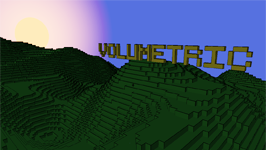
\includegraphics[width=\linewidth]{Volumetric}}
	\vspace{-3mm}

	Group project building a minecraft-esque sandbox game.
\endminipage\hfill
\end{slide}
\vspace{-3mm}
\begin{slide}[H]
\centering
\minipage{0.40\textwidth}
	\fbox{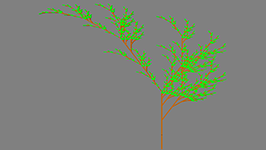
\includegraphics[width=\linewidth]{L-System}}
	\vspace{-3mm}

	Math project using L-Sytems to generate trees
\endminipage\hfill
\minipage{0.40\textwidth}
	\fbox{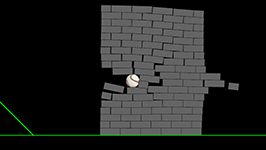
\includegraphics[width=\linewidth]{SFML_Box2D}}
	\vspace{-3mm}

	Tools and Middleware project to integrate different libraries together.
\endminipage\hfill
\end{slide}

\end{document}